
%%%%%%%%%%%%%%%%%%%%%%%%%%%%%%%%%%%%%%%% FIGURE
\begin{figure*}[tb]   
  \begin{center}
   \vspace{-0mm}
   %\includegraphics[width=0.23\textwidth]{figs/model}
   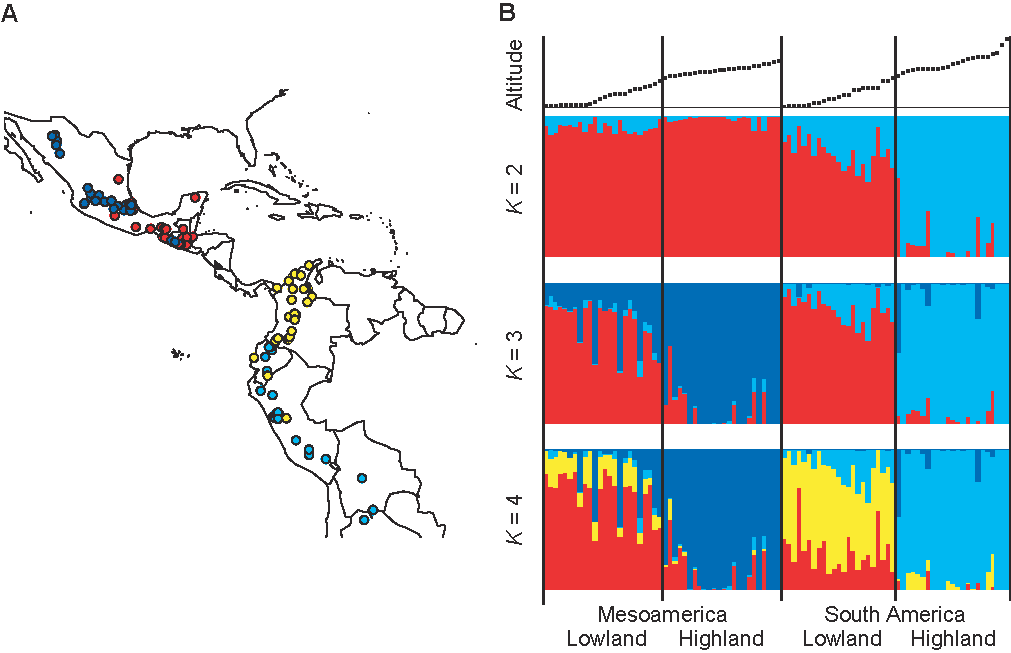
\includegraphics[width=0.8\textwidth]{fig/Fig2}
   \renewcommand{\baselinestretch}{0.9}
   \vspace{-3mm}
   \caption{
   (A) Sampling locations of landraces.  Red, blue, yellow and light blue dots represent Mesoamerican lowland, Mesoamerican highland, S. American lowland and S. American highland populations, respectively.  
   (B) Results of {\sf STRUCTURE} analysis of the maizeSNP50 SNPs with $K=2\sim4$.  The top panel shows the elevation, ranging from 0 to 4,000 m on the \emph{y}-axes.  The colors in $K=4$ correspond to those in panel (A).    }
\vspace{-6mm}
    \label{map}
  \end{center}
\end{figure*}
%%%%%%%%%%%%%%%%%%%%%%%%%%%%%%%%%%%%%%%%% FIGURE

\section*{Materials and Methods}

\subsection*{Materials and DNA extraction}
We included one individual from each of 94 open-pollinated landrace maize accessions from high and low elevation sites in Mesoamerica and S. America (Table \ref{srkid}).   
Accessions were provided by the USDA germplasm repository or kindly donated by Major Goodman (North Carolina State University).  
Sampling locations are shown in Figure~\ref{map}A.  
Landraces sampled from elevations $<1,700$ m were considered lowland, while accessions from $>1,700$ m were considered highland.  
Seeds were germinated on filter paper following fungicide treatment and grown in standard potting mix.  
Leaf tips were harvested from plants at the five leaf stage.  
Following storage at $-80^{\circ}$C overnight, leaf tips were lyophilized for 48 hours.  
Tissue was then homogenized with a Mini-Beadbeater-8 (BioSpec Products, Inc., Bartlesville, OK, USA).  
DNA was extracted using a modified CTAB protocol \cite[]{CTAB}.  
The quality of DNA was ensured through inspection on a 2\% agarose gel and a NanoDrop spectrophotometer (Thermo Scientific, NanoDrop Products, Wilmington, DE, USA).

\subsection*{SNP data}
We generated two complementary SNP data sets for the sampled maize landraces. 
The first set was generated using the Illumina MaizeSNP50 BeadChip platform, including 56,110 SNPs \cite[]{Ganal_2011_22174790}.  
SNPs were clustered with the default algorithm of the GenomeStudio Genotyping Module v1.0 (Illumina Inc., San Diego, CA, USA) and then visually inspected and manually adjusted.   
These data are referred to as ``MaizeSNP50'' hereafter.  
This array contains SNPs discovered in multiple ascertainment schemes \cite[]{Ganal_2011_22174790}, but the vast majority of SNPs come from polymorphisms distinguishing the maize inbred lines B73 and Mo17 (14,810 SNPs) or identified from sequencing 25 diverse maize inbred lines \cite[40,594 SNPs;][]{Gore_2009_19965431}.  

The second data set was generated for a subset of 87 of the landrace accessions (Table~\ref{srkid}) utilizing high-throughput Illumina sequencing data via genotyping-by-sequencing \cite[GBS;][]{Elshire2011}.
Genotypes were called using TASSEL-GBS \cite[]{Glaubitz_GBS} resulting in 2,848,284 SNPs with an average of 71.3\% missing data per individual.

To assess data quality, we compared genotypes at the 7,197 SNPs (229,937 genotypes, excluding missing data) that overlap between the MaizeSNP50 and GBS data sets. 
While only 0.8\% of 173,670  comparisons involving homozygous MaizeSNP50 genotypes differed in the GBS data, 88.6\% of 56,267 comparisons with MaizeSNP50 heterozygotes differed, nearly always being reported as a homozygote in GBS.
Despite this high heterozygote error rate,  the high correlation in allele frequencies between data sets ($r=0.89$; Figure~\ref{supp:correl_freq}) supports the utility of the GBS data set for estimating allele frequencies.  

We annotated SNPs using the filtered gene set from RefGen version 2 of the maize B73 genome sequence (\citealt{Schnable_2009_19965430}; release 5b.60) from maizesequence.org.  
We excluded genes annotated as transposable elements (84) and pseudogenes (323) from the filtered gene set, resulting in a total of 38,842 genes.

\subsection*{Structure analysis}
We performed a {\sf STRUCTURE} analysis \cite[]{Pritchard_2000_10835412,Falush_2003_12930761} using \rev{only} synonymous and noncoding SNPs from the MaizeSNP50 data \rev{due to its low error in identifying heterozygous genotypes}. 
We randomly pruned SNPs closer than 10 kb and assumed free recombination between the remaining SNPs.
Alternative distances were tried with nearly identical results. 
We excluded SNPs in which the number of heterozygous individuals exceeded homozygotes and where the \emph{P}-value for departure from Hardy-Weinberg Equilibrium (HWE) using all individuals was smaller than 0.05 based on a \emph{G}-test. 
Following these data thinning measures, 17,013 biallelic SNPs remained. 
We conducted three replicate runs of {\sf STRUCTURE} using the correlated allele frequency model with admixture for \emph{K} = 2 through \emph{K} = 6 populations, a burn-in length of 50,000 iterations and a run length of 100,000 iterations. 
Results across replicates were nearly identical.

\subsection*{Historical population size}
We tested three models in which maize was differentiated into highland and lowland populations subsequent to domestication (Figure~\ref{model}). 

\rev{We calculated the observed joint frequency distributions (JFDs) using only} the GBS data set due to its lower level of ascertainment bias. 
A subset of synonymous and noncoding SNPs were utilized that had $\geq15$ individuals without missing data in both lowland and highland populations and did not violate HWE.  
A HWE cut-off of $P<0.005$ was used for each subpopulation due to our under-calling of heterozygotes. 

%\plrnote{this next sentence is confusing.  can just delete the ``for the X populations'', as this is explained later?}
%In total, we included 18,745 synonymous and noncoding SNPs for the Mesoamerican populations in Models IA and IB, 14,508 for the S. American populations in Model I and 11,305 for the Mesoamerican lowland population and the S. American populations in Model II.  
We obtained similar results under more or less stringent thresholds for significance ($P < 0.05 \sim 0.0005$; data not shown), though the number of SNPs was very small at $P<0.05$.  

Parameters were inferred with the software $\delta a \delta i$ \cite[]{Gutenkunst_2009_19851460}, which uses a diffusion method to calculate an expected JFD and evaluates the likelihood of the data assuming multinomial sampling. We did not use the ``full'' model that incorporates all four populations because parameter estimation under this model is computationally infeasible.

%%%%%%%%%%%%%%%%%%%%%%%%%%%%%%%%%%%%%%%%% FIGURE
\begin{figure}[tb]   
  \begin{center}
   \vspace{-0mm}
   %\includegraphics[width=0.23\textwidth]{figs/model}
   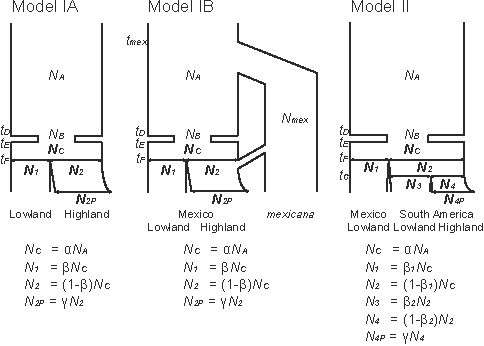
\includegraphics[width=0.5\textwidth]{fig/Fig3}
   \renewcommand{\baselinestretch}{0.9}
   \vspace{-3mm}
   \caption{  Models of historical population size for lowland and highland populations.  Parameters in bold were estimated in this study.  See text for details.
   }
\vspace{-6mm}
    \label{model}
  \end{center}
\end{figure}
%%%%%%%%%%%%%%%%%%%%%%%%%%%%%%%%%%%%%%%%% FIGURE

\paragraph{Model IA}
This model is applied separately to both the Mesoamerican and the S. American populations.
We assume the ancestral diploid population representing \emph{parviglumis} follows a standard Wright-Fisher model with constant size.  
The size of the ancestral population is denoted by $N_A$.
At $t_D$ generations ago, the bottleneck event begins at domestication, and at $t_E$ generations ago, the bottleneck ends.  
The population size and duration of the bottleneck are denoted by $N_B$ and $t_B=t_D-t_E$, respectively.  
The population size recovers to $N_C=\alpha N_A$ in the lowlands.  
Then, the highland population is differentiated from the lowland population at $t_F$ generations ago.  
The size of the lowland and highland populations at time $t_F$ is determined by a parameter $\beta$ such that the population is divided by $\beta N_C$ and $(1-\beta)N_C$; our conclusions hold if we force lowland population size to remain at $N_C$ (data not shown).  

We assume that the population size in the lowlands is constant but that the highland population experiences exponential expansion after divergence: its current population size is $\gamma$ times larger than that at $t_F$. \\

\paragraph{Model IB}
We expand Model IA for the Mesoamerican populations by incorporating admixture from the teosinte \emph{mexicana} to the highland Mesoamerican maize population.  
The time of differentiation between \emph{parviglumis} and \emph{mexicana} occurs at $t_{mex}$ generations ago.  
The \emph{mexicana} population size is assumed to be constant at $N_{mex}$.  
At $t_F$ generations ago, the Mesoamerican highland population is derived from admixture between the Mesoamerican lowland population and a portion $P_{mex}$ from the teosinte \emph{mexicana}.\\  

\paragraph{Model II}
The final model includes the Mesoamerican lowland, S. American lowland and highland populations.  
This model was used for simulating SNPs with ascertainment bias (see below).  
At time $t_F$, the Mesoamerican and S. American lowland populations are differentiated, and the sizes of populations after splitting are determined by $\beta_1$.  
At time $t_G$, the S. American lowland and highland populations are differentiated, and the sizes of populations at this time are determined by $\beta_2$.  
As in Model IA, the S. American highland population is assumed to experience population growth with the parameter $\gamma$.\\

Estimates of a number of our model parameters were available from previous work.    
$N_A$ was set to 150,000 using estimates of the composite parameter $4N_A\mu \sim 0.018$ from \emph{parviglumis}  \cite[]{Eyre-Walker_1998_9539756,Tenaillon_2001_11470895,Tenaillon_2004_15014173,Wright_2005_15919994,Ross-Ibarra_2009_19153259} and an estimate of the mutation rate $\mu \sim 3\times 10^{-8}$ \cite[]{Clark_2005_16079248} per site per generation.  
The severity of the domestication bottleneck is represented by $k=N_B/t_B$ \cite[]{Eyre-Walker_1998_9539756,Wright_2005_15919994}, and following \cite{Wright_2005_15919994} we assumed $k=2.45$ and $t_B=1,000$ generations.  
Taking into account archaeological evidence \cite[]{Piperno_2009_19307570}, we assume $t_D=9,000$ and $t_E=8,000$.  
We further assumed $t_F=6,000$ for Mesoamerican populations in Models IA and IB \cite[]{Piperno_2006_69}, $t_F=4,000$ for S. American populations in Model IA \cite[]{Perry_2006_16511492,Grobman_2012_22307642}, and $t_{mex}=60,000$, $N_{mex}=160,000$ \cite[]{Ross-Ibarra_2009_19153259}, and $P_{mex}=0.2$ \cite[]{vanHeerwaarden_2011_21189301} for Model IB. 
For both Models IA and IB, we inferred three parameters ($\alpha$, $\beta$ and $\gamma$), and, for Model II, we fixed $t_F=6,000$ and $t_G=4,000$ \cite[]{Piperno_2006_69,Perry_2006_16511492,Grobman_2012_22307642}  and estimated the remaining four parameters ($\alpha$, $\beta_1$, $\beta_2$ and $\gamma$).

\subsection*{Population differentiation}
We used our inferred models of population size change to generate a null distribution of $F_{ST}$.
As implemented in $\delta a \delta i$ \cite[]{Gutenkunst_2009_19851460}, we calculated an expected JFD given estimated model parameters and the sample sizes from our highland and lowland populations.
Then, we converted the JFD into the distribution of $F_{ST}$ values.
The \emph{P}-value of a SNP was calculated by $P(F_{ST\_E}\geq F_{ST\_O}|p\pm 0.025) = P(F_{ST\_E}\geq F_{ST\_O} \cap p\pm 0.025)/P(p\pm 0.025)$, 
where $F_{ST\_O}$ and $F_{ST\_E}$ are observed and expected $F_{ST}$ values and $p\pm 0.025$ is the set of loci with mean allele frequency across both highland and lowland populations within 0.025 of the SNP in question. 

Generating the null distribution of differentiation for the MaizeSNP50 data requires accounting for ascertainment bias. 
Evaluation of genetic clustering in our data (not shown) coincides with previous work \cite[]{Hufford_2012_22660546} in suggesting that the two inbred lines most important in the ascertainment panel (B73 and Mo17) are most closely related to Mesoamerican lowland maize.  
We thus added two additional individuals to the Mesoamerican lowland population and generated our null distribution using only SNPs for which the two individuals had different alleles.
For model IA in S. America we added two individuals at time $t_F$ to the ancestral population of the S. American lowland and highland populations because the Mesoamerican lowland population was not incorporated into this model. 
For each combination of sample sizes in lowland and highland populations, we generated a JFD from $10^7$  SNPs using the software {\sf ms} \cite[]{Hudson_2002_11847089}.
Then, we calculated \emph{P}-values from the JFD in the same way.
We calculated $F_{ST}$ values for all SNPs that had $\geq10$ individuals with no missing data in all four populations and showed no departure from HWE at the 0.5\% (GBS) or 5\% (MaizeSNP50) level. 

%\jri{we don't correct for allele frequency (or heterozygosity) in our Fst outlier analysis do we?  if not, this is a problem I think.}
%\st{I did.  No essential change}

%\jri{do we use all GBS data in the Fst outlier test, or just silent SNPs? we should be able to use nonsynonymous too, right?}
%\st{I used all.}

\subsection*{Haplotype sharing test}
We performed a \underline{p}airwise \underline{h}aplotype \underline{s}haring (PHS) test to detect further evidence of selection, following \cite{Toomajian_2006_16623598}.  
To conduct this test, we first imputed and phased the combined SNP data (both GBS and MaizeSNP50) using the {\sf fastPHASE} software version 1.4.0 \cite[]{Scheet_2006_16532393}.  
As a reference for phasing, we used data (excluding heterozygous SNPs) from an Americas-wide sample of 23 partially inbred landraces from the Hapmap v2 data set  \cite[]{Chia_2012_22660545}.  
We ran {\sf fastPHASE}  with default parameter settings.  
PHS was calculated for an allele \emph{A} at position $x$ by

%  \displaystyle{
%PHS_{x_A} = \sum^{p-1}_{i=1}\sum^{p}_{j=i+1}Z_{ijx}  / \Bigl( \begin{array}{c} p \\ 2 \\ \end{array} \Bigr) 
%- \sum^{n-1}_{i=1}\sum^{n}_{j=i+1}Z_{ijx}  / \Bigl( \begin{array}{c} n \\ 2 \\ \end{array} \Bigr) 
%  }

\begin{equation}
  \label{phs-1}
  \begin{array}{l}
  \displaystyle{
PHS_{x_A} = \sum^{p-1}_{i=1}\sum^{p}_{j=i+1} \frac{ Z_{ijx} }{ {p \choose 2} } - \sum^{n-1}_{i=1}\sum^{n}_{j=i+1} \frac{ Z_{ijx}  }{ {n \choose 2}}
  }
  \end {array} 
  \textrm{,}
\end{equation}
\noindent where $n$ is the sample size of haploids, $p$  is the number of haploids carrying the allele $A$ at position $x$, and

\begin{equation}
  \label{phs-2}
  \begin{array}{l}
  \displaystyle{
Z_{ijx} = \frac{ d_{ijx} - \bar{d_{ij}} }{ \sigma_{ij} }
  }
  \end {array} 
  \textrm{,}
\end{equation}
\noindent where $d_{ijx}$ is the genetic distance over which individuals $i$ and $j$ are identical surrounding position $x$, 
$\bar{d_{ij}}$ is the genome-wide mean of distances over which individuals $i$ and $j$ are identical, 
and $\sigma_{ij}$ is the standard deviation of the distribution of distances.  
To identify outlying PHS values, we used the empirical quantile, calculated as the proportion of alleles of the same frequency genome-wide that have a larger PHS value; \st{we calculated Pr($PHS_{xA}\leq PHS_{null|p}$), where $PHS_{null|p}$ is PHS values for alleles in frequency, $p$.  The smaller the statistics is, the longer the length of a haplotype around the allele is}.

Genetic distances were obtained for the MaizeSNP50 data \citep{Ganal_2011_22174790} and fit using a tenth degree polynomial curve to all SNPs (data not shown).

%%%% PLR:
\subsection*{Theoretical evaluation of convergent evolution }

\rev{
We now turn to theory
to assess whether the abundance and degree of coincidence of presumably adaptive high-$F_{ST}$ alleles is consistent with what is known about the population history of maize.
There are three ways that adaptive alleles could be shared between highland populations:
(a) by appearing in both locations as independent, \textit{de novo} mutations;
(b) by moving from one highland population to the other my migration;
and 
(c) through convergent selective forces acting on shared standing variation.
In the text we provide fairly rough estimates,
and develop more detailed, complementary models 
that build on the work in \citet{ralph2014convergent} and \citet{ralph2014standing}
in the Appendix.
% PLR: to explain why we are using a complicated model.
Much of the population genetics theory we use
relies on universality results that reduce demographic models
to two parameters: the dispersal distance (mean parent-offspring distance),
and the variance in offspring number.
However, these universality results do not hold if either distribution
(of dispersal distribution or of offspring number)
is sufficiently long-tailed,
so we chose to implement a fairly detailed demographic model
to both get a good idea of what part of parameter space we should focus on,
and to verify that the approximation results we use are good.
}

To assess the likely importance of (a) and (b),
we first evaluate the rate at which we expect an allele that provides a selective advantage at higher elevation to arise by new mutation in \rev{or near} a highland region ($\mutrate$), 
and then use coalescent theory to show that even a highland-adapted allele that was neutral in the lowlands
is unlikely to have had time to spread between highland populations under neutral gene flow.
\rev{
It may be more likely that alleles adapted in the highlands are slightly deleterious at lower elevation, 
consistent with empirical findings in reciprocal transplant experiments in Mexico \cite[]{Mercer2008};
in the Appendix we find the rate at which such an allele already present in the Mesoamerican highlands would transit the intervening lowlands and fix in the Andean highlands.
The resulting values depend most strongly on the population density, the selection coefficient, and the rate at which seed is transported long distances and replanted; 
\jri{add text about how likely this is, cite JvH and emprical estimates}
we checked the results by evaluating several choices of these parameters as well as with simulations, described in the Appendix.
Here we describe the mathematical details; 
readers may skip to the results without loss of continuity.
}

\paragraph{Demographic model}
Throughout, we followed \citet{vanHeerwaarden2010} in constructing a detailed demographic model for domesticated maize.
We assume fields of $N=10^5$ plants are replanted each year from $N_f=561$ ears, either from completely new stock (with probability $p_e=0.068$), from partially new stock (a proportion $r_m=0.2$ with probability $p_m=0.02$), or  otherwise entirely from the same field.
Each plant is seed parent to all kernels of its own ears, but can be pollen parent to kernels in many other ears; a proportion $m_g=0.0083$ of the pollen-parent kernels are in other fields.
Wild-type plants have an average of $\mu_E=3$ ears per plant, and ears have an average of $N/N_f$ kernels; each of these numbers are Poisson distributed.
The mean number of pollen-parent kernels, and the mean number of kernels per ear, is assumed to be $(1+s_b)$ times larger for individuals heterozygous for the selected allele.
(The fitness of homozygotes is assumed to not affect the probability of establishment.)
Migration is mediated by seed exchange -- when fields are replanted from new stock, the seed is chosen from a random distance away with mean $\sigma_s=50$km, but plants only pollinate other plants belonging to the same village (distance 0).
The mean numbers of each category of offspring (seed/pollen; migrant/nonmigrant) are determined by the condition that the population is stable 
(i.e., wild-type, diploid individuals have on average 2 offspring) 
except that heterozygotes have on average $(1+s_b)$ offspring that carry the selected allele.
Each ear has a small chance of being chosen for replanting, so the number of ears replanted of a given individual is Poisson, and assuming that pollen is well-mixed, the number of pollen-parent kernels is Poisson as well.
Each of these numbers of offspring has a mean that depends on whether the field is replanted with new stock, and whether ears are chosen from this field to replant other fields, so the total number of offspring is a mixture of Poissons. 
These means, and more details of the computations, are found in the Appendix. % \ref{apx:demographic_model}.}
At the parameter values given, 
the dispersal distance (mean distance between parent and offspring) is $\sigma=3.5$km,
\rev{
and the haploid variance in number of offspring 
($\xi^2$, the variance in number of inherited copies of a chosen parental allele)
}
is between 20 (for wild-type) and 30 (for $s_b=0.1$).
\rev{
(Note that in a panmictic population, the offspring variance
is approximately the ratio of census size to effective population size, $\xi^2 \approx N/N_e$.)
}

\paragraph{New mutations}
The rate at which new mutations appear and fix in a highland population, which we denote $\mutrate$, 
is approximately equal to the total population size of the highlands multiplied by the mutation rate per generation 
and the chance that a single such mutation successfully fixes (i.e., is not lost to drift).
The probability that a single new mutant allele providing benefit $s_b$ to heterozygotes at high elevation 
will fix locally in the high elevation population is approximately $2s_b$ divided by the 
\rev{
haploid variance in offspring number 
(by expanding the generating function near 1, as in \citep{fisher1922dominance,jagers1975branching}; see \citet{lambert2006probability} for more sophisticated models).
}

Concretely, the probability that a new mutation destined for fixation will arise in a patch of high-elevation habitat of area $A$ in a given generation is a function of the density of maize per unit area $\rho$, the selective benefit $s_b$ it provides, the mutation rate $\mu$, and the variance in offspring number $\xi^2$.
In terms of these parameters, the rate of appearance is 
\begin{align} \label{eqn:mutrate}
  \mutrate = \frac{2 \mu \rho A s_b}{\xi^2} .
\end{align}

\rev{
\paragraph{Geographic distribution}
Throughout we work with populations distributed continuously across geography,
with two regions of high elevation, the Mesoamerican and Andean highlands, separated by about 4,000km.
The value $A$ in equation \eqref{eqn:mutrate} is the total cultivated area in which the (highland-adapted) alleles in question are beneficial;
for estimation of $A$ in South America we overlaid raster layers of altitude (\url{www.worldclim.org}) and extent of maize cultivation (\url{www.earthstat.org}) and calculated the total area of maize cultivated above 1700m using functions in the {\sf raster} package for {\sf R}.
}

\rev{
Of course, the selective benefit of highland alleles is not discrete, but likely changes continuously with altitude,
and it may be that the adaptive mutation occurs in a lowland area,
subsequently migrating into the highlands.
The calculation above does account for these points,
but the approximation is quite good,
as verified by exact numerical calculation of the chance of fixation of a mutation 
as a function of the location where it first appears (see Figure~\ref{sfig:prob_estab}); 
for theoretical treatment see \citet{barton1987establishment}.
}

\paragraph{Migration}
It is harder to intuit
a corresponding expression for the chance that an allele established by selection in one highland population moves to the other.

For maize in the Andean highlands to have inherited a highland-adapted allele from the Mesoamerican highlands, 
those Andean plants must be directly descended from highland Mesoamerican plants that lived more recently than the appearance of the adaptive allele.
In other words, the ancestral lineages along which the modern Andean plants have inherited at that locus must trace back to the Mesoamerican highlands.
If the allele is neutral in the lowlands, we can treat the movement of these lineages as a neutral process, using the framework of coalescent theory 
\citep{wakeley2005coalescent}.
To do this, we need to follow \emph{all} of the $N \approx 2.5 \times 10^6$ lineages backwards.
These quickly coalesce to fewer lineages;
but this turns out to not affect the calculation much.
% these quickly coalesce to fewer $m$ lineages in approximately $\sum_{k=m}^N \frac{2N}{\xi^2 k(k+1)} \approx 1.25 \times 10^5/m$ generations, leaving about 1000 lineages after 100 generations that are spread over a larger area.
Assuming demographic stationarity,
the motion of each lineage can be modeled as a random walk,
whose displacement after $m$ generations has variance $m \sigma^2$, and for large $m$ is approximately Gaussian.
If we assume that lineages move independently, 
and $Z_n$ is the distance to the furthest of $n$ lineages, 
then $Z_n \le \sqrt{m \sigma^2} ( \sqrt{2 \log n} + \sqrt{2/\log n} )$ with very high probability
% then $\P\{ Z_n / \sqrt{m \sigma^2} \le x /\sqrt{2 \log n} + \sqrt{2 \log n} - (1/2) (\log \log n + \log 4 \pi)/\sqrt{2 \log n} \} \approx \exp( - e^{-x} )$ 
\citep{berman1964limit}. 

Since this depends only on the logarithm of $n$, the number of lineages,
the practical upshot of this is that the most distant lineage
is very unlikely to be more than about 6 times more distant than the typical lineage,
even among $10^7$ lineages.
Lineages are not independent, but this only makes this calculation conservative.
Therefore, an area today (say, the Andean highlands)
is very unlikely to draw any ancestry from a region more than about $6 \sigma \sqrt{m}$ kilometers away from $m$ generations ago
in a part of the genome that is neutral in the lowlands;
with $m=4000$ and $\sigma=3.5$km this is 1,328km.

% # code to verify this: (and, see maize_calcs.R to verify this random walk is close to Gaussian after 2,000 generations)
% x <- rnorm(1e6)  # independent
% # x <- rnorm(1e6,sd=1/sqrt(2),mean=rep(rnorm(1e3,sd=1/sqrt(2)))) # or, correlated
% nvals <- 1e3*(1:(length(x)/1e3))
% maxvals <- cummax(x)[nvals]
% meanvals <- sqrt(2*log(nvals))-(1/2)*(log(log(nvals))+log(4*pi))/sqrt(2*log(nvals)) 
% # 95% quantile:
% exp.95 <- log(1/log(1/.95))/sqrt(2*log(nvals)) + meanvals
% # 5% quantile:
% exp.05 <- log(1/log(1/.05))/sqrt(2*log(nvals)) + meanvals
% plot( nvals, maxvals, ylim=range(maxvals,exp.95,exp.05) )
% lines( nvals, meanvals )
% lines( nvals, exp.95, lty=2 )
% lines( nvals, exp.05, lty=2 )
% lines( nvals, sqrt(2*log(nvals))+2/sqrt(2*log(nvals)), col='red' )

